\chapter{Some extra stuff}
\label{AppendixA}

\section{Marginal Abatement Cost Curve}
\label{sec:MACC}


% \section{Financial Predictors Full-Size Graphs}
% \label{sec:FinancialPreds}

% \begin{figure}[H]
% \centering
% \subcaptionbox{Total Assets\label{fig:total-assets}}{%
%   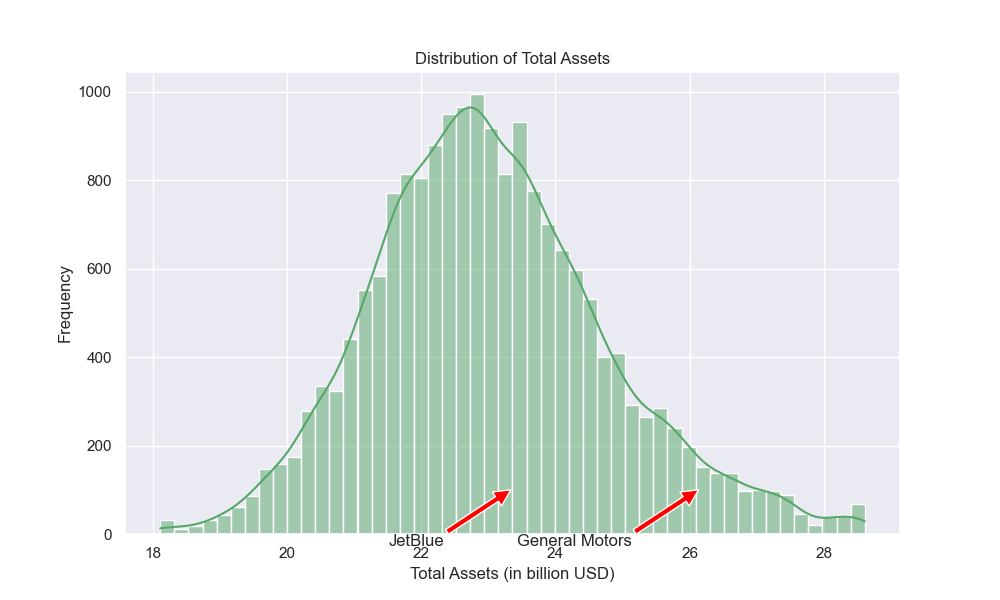
\includegraphics[width=0.8\textwidth]{figures/financial_preds/tot_assets_dist.png}}
% \caption{Financial Predictors: Total Assets}
% \end{figure}

% \begin{figure}[H]
% \centering
% \subcaptionbox{Market Capitalization\label{fig:market-capitalization}}{%
%   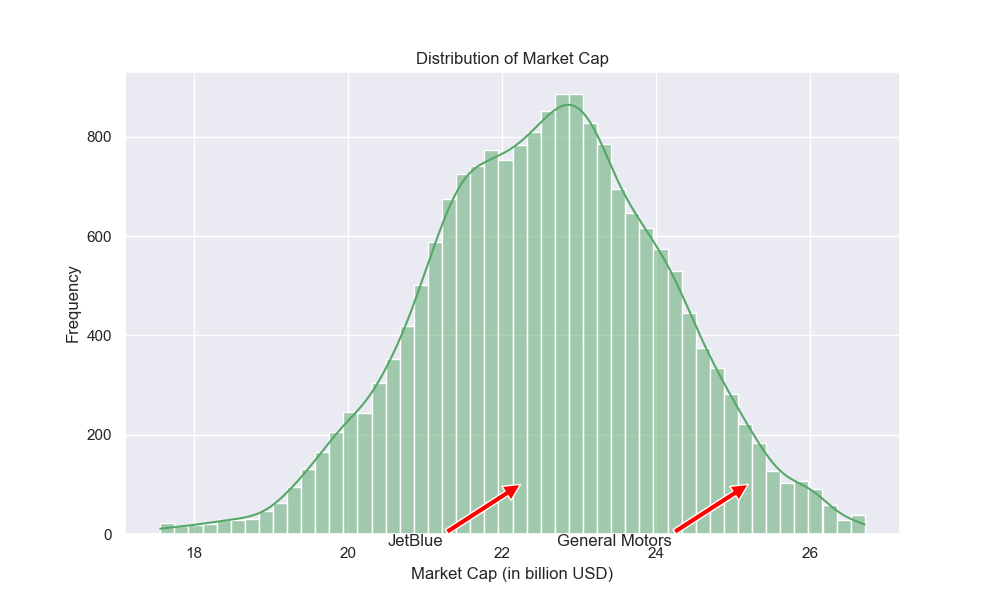
\includegraphics[width=0.8\textwidth]{figures/financial_preds/mkt_cap_dist.png}}
% \caption{Financial Predictors: Market Capitalization}
% \end{figure}

% \begin{figure}[H]
% \centering
% \subcaptionbox{Return on Equity\label{fig:roe}}{%
%   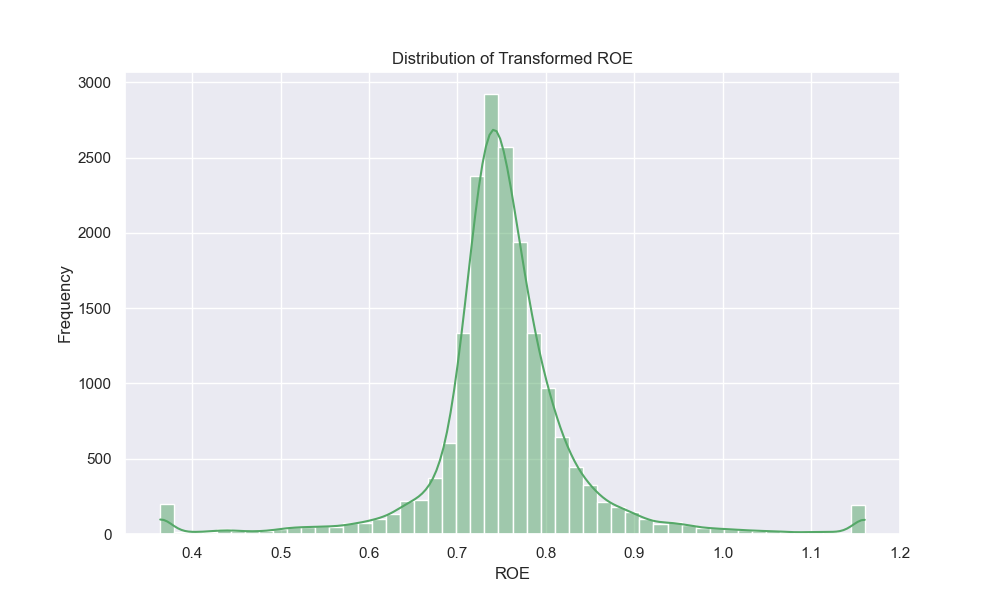
\includegraphics[width=0.8\textwidth]{figures/financial_preds/roe_dist.png}}
% \caption{Financial Predictors: Return on Equity}
% \end{figure}

% \begin{figure}[H]
% \centering
% \subcaptionbox{Revenue\label{fig:revenue}}{%
%   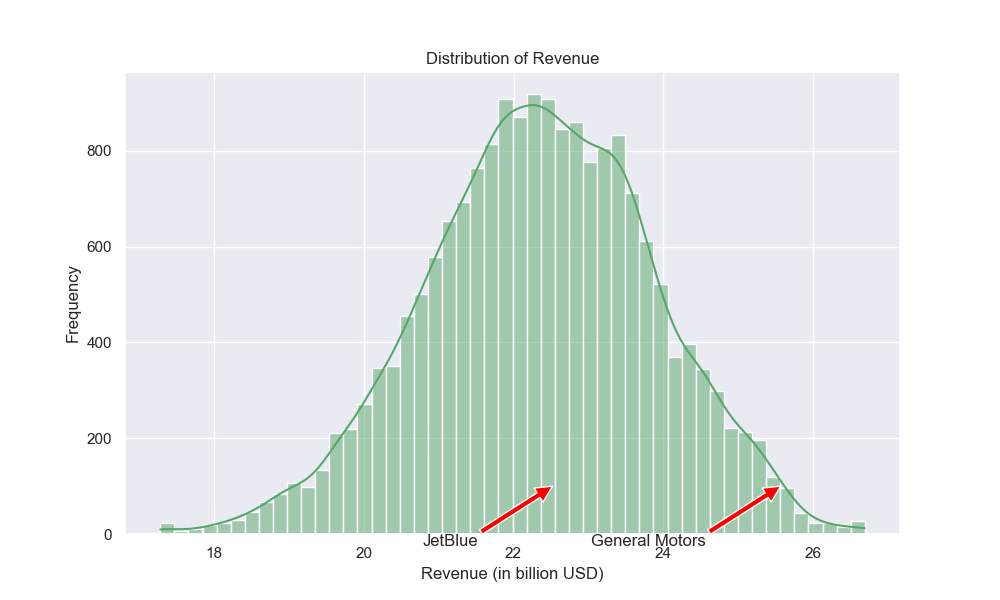
\includegraphics[width=0.8\textwidth]{figures/financial_preds/revenue_dist.png}}
% \caption{Financial Predictors: Revenue}
% \end{figure}

% \begin{figure}[H]
% \centering
% \subcaptionbox{Net Income\label{fig:net-income}}{%
%   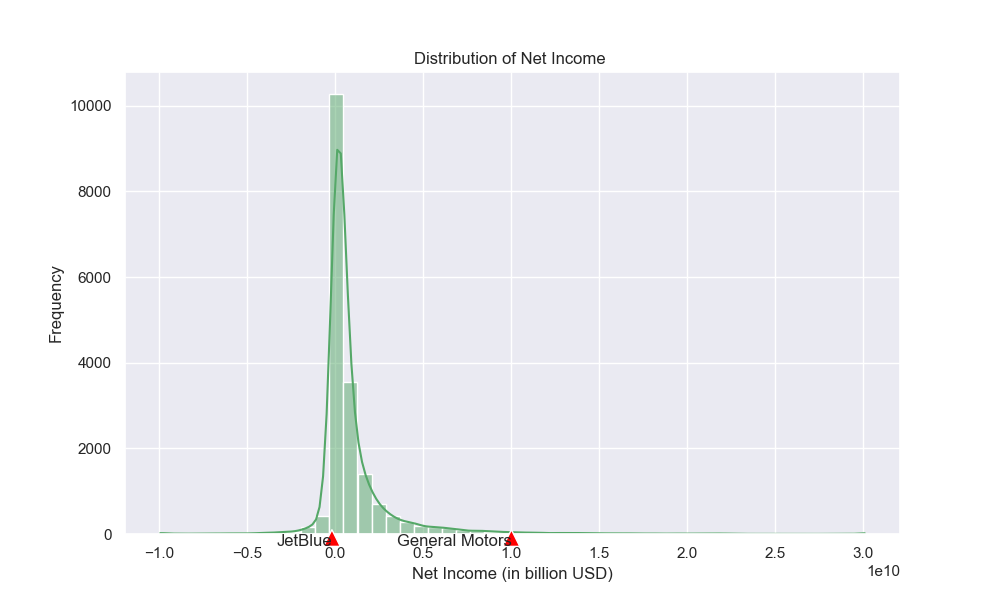
\includegraphics[width=0.8\textwidth]{figures/financial_preds/net_income_dist.png}}
% \caption{Financial Predictors: Net Income}
% \end{figure}

% \begin{figure}[H]
% \centering
% \subcaptionbox{Employees\label{fig:employees}}{%
%   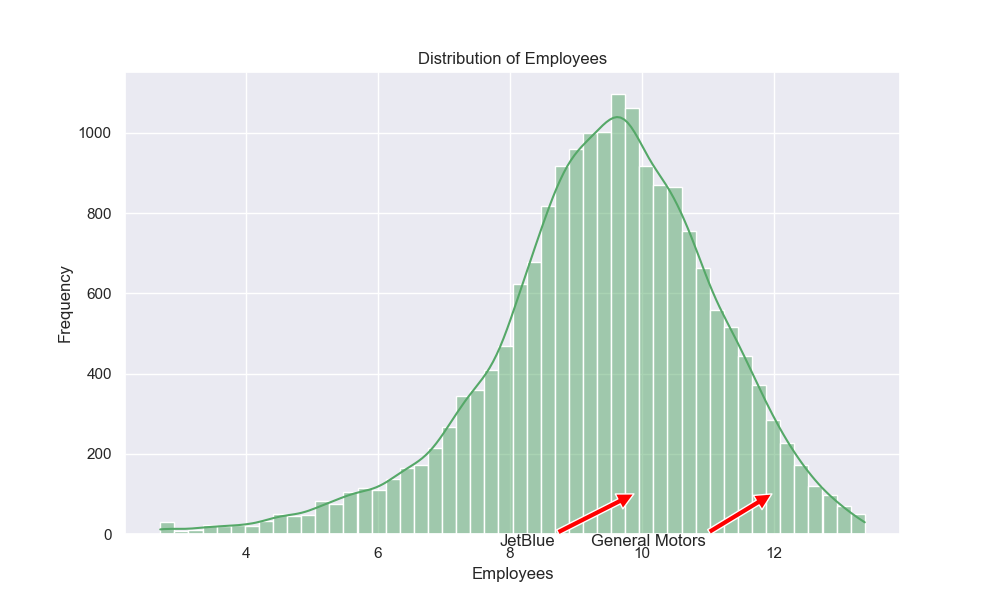
\includegraphics[width=0.8\textwidth]{figures/financial_preds/employees_dist.png}}
% \caption{Financial Predictors: Employees}
% \end{figure}

% \begin{figure}[H]
% \centering
% \subcaptionbox{Total Assets 1yr Growth\label{fig:total-assets-1yr-growth}}{%
%   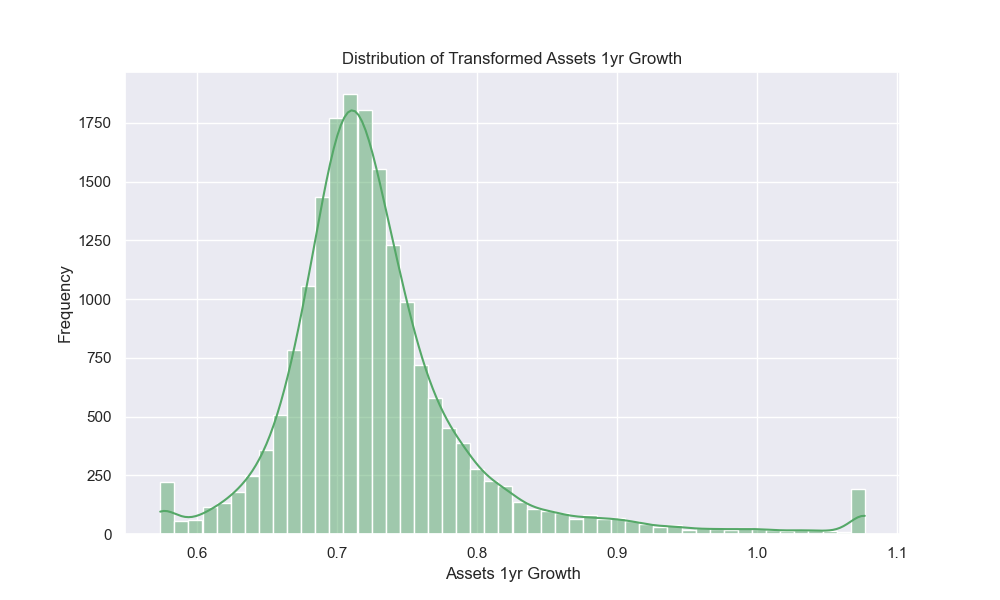
\includegraphics[width=0.8\textwidth]{figures/financial_preds/assets_1yr_growth_dist.png}}
% \caption{Financial Predictors: Total Assets 1yr Growth}
% \end{figure}

% \begin{figure}[H]
% \centering
% \subcaptionbox{Employees 1yr Growth\label{fig:employees-1yr-growth}}{%
%   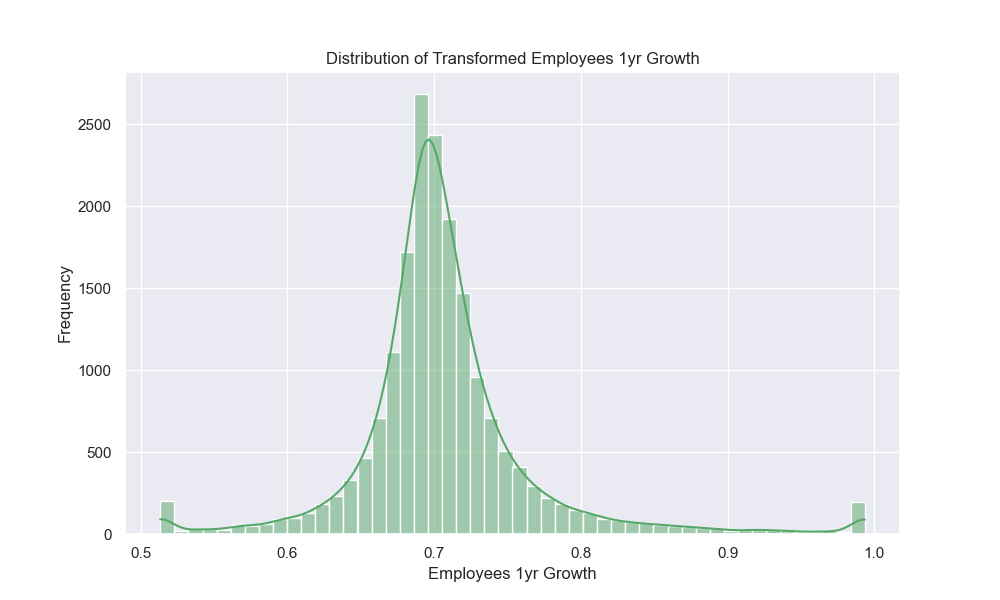
\includegraphics[width=0.8\textwidth]{figures/financial_preds/employees_1yr_growth_dist.png}}
% \caption{Financial Predictors: Employees 1yr Growth}
% \end{figure}

% \begin{figure}[H]
% \centering
% \subcaptionbox{Net Income Over Assets\label{fig:net-income-over-assets}}{%
%   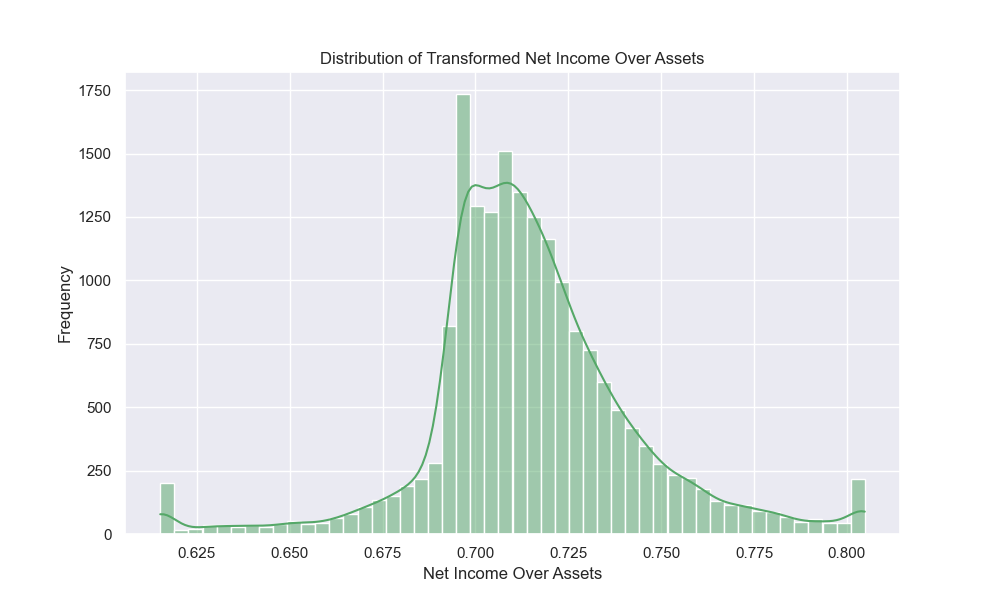
\includegraphics[width=0.8\textwidth]{figures/financial_preds/net_income_over_assets_dist.png}}
% \caption{Financial Predictors: Net Income Over Assets}
% \end{figure}


%  \setlength{\tabcolsep}{4pt}
%  \renewcommand{\arraystretch}{2.4}
% \footnotesize
% \begin{center}
%   \begin{tabular}{lcccc}
%     \hline
%  \textbf{Name} & \textbf{Param.} & \textbf{PMF or PDF} & \textbf{Mean} & \textbf{Variance} \\ 
%     \hline
%     Bernoulli & $p$ & $P(X=1) =p, P(X=0) = q$ & $p$ & $pq$ \\ 
%     Binomial & $n,p$ & ${n \choose k} p^k q^{n-k},   \,k \in \{0,1,\dots,n\}$ & $np$ & $npq$\\ 
%     FS & $p$ & $pq^{k-1},  \,k \in \{1,2,\dots\}$& $1/p$ & $q/p^2$\\ 
%     Geom & $p$ & $pq^{k},   \,k \in \{0,1,2,\dots\}$& $q/p$ & $q/p^2$\\ 
%     NBin & $r, p$ &  ${r+k-1 \choose r-1} p^r q^{k},  \,k \in \{0,1,2,\dots\}$ & $rq/p$ & $rq/p^2$ \\ 
%      HGeom & $w,b,n$ & $\frac{{w \choose k}{b \choose n-k}}{{{w+b} \choose n}}, \,k \in \{0,1,\dots,n\}$ & $\mu = \frac{nw}{w+b}$ & $(\frac{w+b-n}{w+b-1}) \mu (1-\frac{\mu}{n})$\\
%       NHGeom & $w,b,r$ & $ \frac{{r+k-1 \choose {r-1}}{w+b-r-k \choose w-r}}{{ {w+b} \choose {w}}},  \, k \in \{0,1,\dots,b\}$ & $\frac{rb}{w+1}$ & $ \frac{rb(w+b+1)(w-r+1)}{(w+1)^2(w+2)}$\\
%     Poisson & $\lambda$ & $\frac{e^{-\lambda} \lambda^k}{k!},  \,k \in \{0,1,2,\dots\}$ & $\lambda$ & $\lambda$ \\ 
%     Uniform & $a < b$ & $\frac{1}{b-a},   \,x \in (a,b)$ & $\frac{a+b}{2}$& $\frac{(b-a)^2}{12}$ \\ 
%     Normal & $\mu, \sigma^2$ & $\frac{1}{\sigma \sqrt{2\pi}}e^{-(x - \mu)^2/(2\sigma^2)}$ & $\mu$ & $\sigma^2$ \\ 
%     Log-Normal  &  $\mu, \sigma^2$ & $\frac{1}{x\sigma \sqrt{2\pi}}e^{-(\log x - \mu)^2/(2\sigma^2)},\, x > 0$ & $\theta = e^{ \mu + \sigma^2/2}$ & $\theta^2 (e^{\sigma^2} - 1)$\\
%     Expo & $\lambda$ &  $\lambda e^{-\lambda x}, \,x > 0$& $1/\lambda$ & $1/\lambda^2$ \\ 
%         Weibull & $\lambda, \gamma$ &  $ \gamma \lambda e^{-\lambda x^\gamma} x^{\gamma -1},  \,x > 0$& $\mu = \frac{\Gamma\left(1+1/\gamma \right)}{\lambda^{1/\gamma}}$ & $\frac{\Gamma\left(1 + 2/\gamma \right)}{\lambda^{2/\gamma}} - \mu^2$ \\ 
%     Gamma & $a, \lambda$ &  $\Gamma(a)^{-1} (\lambda x)^a e^{-\lambda x} x^{-1},  \,x > 0$& $a/\lambda$ & $a/\lambda^2$ \\ 
%     Beta & $a, b $ & $\frac{\Gamma(a + b)}{\Gamma(a)\Gamma(b)} x^{a-1}(1-x)^{b-1}, \,0<x<1$ & $\mu = \frac{a}{a+b}$ & $\frac{\mu (1-\mu)}{a+b+1}$\\
%    Chi-Square & $n$ & $\frac{1}{2^{n/2}\Gamma(n/2)}x^{n/2-1}e^{-x/2},  \,x>0$ & $n$ & $2n$\\
%     Student-$t$ & $n$ & $\frac{\Gamma((n+1)/2)}{\sqrt{n\pi} \Gamma(n/2)} (1+x^2/n)^{-(n+1)/2}$ & 0 if $n>1$ & $\frac{n}{n-2}$ if $n>2$\\
%     \hline
%   \end{tabular}
% \end{center}
% \normalsize


\section{Variable Dictionary}
\label{sec:variable-dictionary}

\noindent Table~\ref{tab:variable-dictionary} provides an overivew of the predictors used in the analysis, including their type, description, and source. Predictors are divided into three primary categories: \begin{itemize}
    \item \textbf{Firm Information:} Variables that describe the firm's characteristics, such as its unique identifier, reporting year, headquarters country, headquarters continent, and industry sector.
    \item \textbf{Financial Predictors:} Variables that capture the firm's financial performance, including total revenue, total assets, total employees, net income, and market capitalization.
    \item \textbf{CDP Predictors:} Variables derived from the CDP Climate Survey, such as the firm's emissions, energy consumption, and climate-related targets and initiatives.
\end{itemize}


\begin{longtable}{lp{2cm}p{5cm}p{2cm}} \\
    \toprule
    \textbf{Variable} & \textbf{Type} & \textbf{Description} & \textbf{Source} \\
    \midrule
    \endfirsthead % Everything above goes at the top of the first page of the table
    \multicolumn{4}{c}%
    {\tablename\ \thetable\ -- \textit{Continued from previous page}} \\
    \toprule
    \textbf{Variable} & \textbf{Type} & \textbf{Description} & \textbf{Source} \\
    \midrule
    \endhead % Header to be repeated on every page
    \bottomrule
    \multicolumn{4}{r}{\textit{Continued on next page}} \\
    \endfoot % Footer to be repeated on every page except the last
    \endlastfoot % Footer for the last page of the table
    
    % Core Information Section
    \multicolumn{4}{l}{\textbf{Firm Information}} \\
    \midrule
    ID & categorical & unique firm identifier & CDP \\
    Year & numerical & reporting year & CDP \\
    Country & categorical & headquarters country  & CDP \\
    Continent & categorical & headquarters continent derived from country & CDP \\
    Industry & categorical & Global Industry Classification Standard 25 industry sectors & GICS \\
    
    \midrule
    % Financial Predictors Section
    \multicolumn{4}{l}{\textbf{Financial Predictors}} \\
    \midrule
    log(Revenue) & numerical & natural logarithm of total revenue & Worldscope \\
    log(Assets) & numerical & natural logarithm of total assets & Worldscope \\
    log(Assets 1yr gr.) & numerical & natural logarithm of total assets growth & Worldscope \\
    log(Employees) & numerical & natural logarithm of total employees & Worldscope \\
    log(Empl. 1y gr.) & numerical & natural logarithm of total employees growth & Worldscope \\
    log(Net Income) & numerical & natural logarithm of net income & Worldscope \\
    log(Market Cap) & numerical & market capitalization & Worldscope \\
    log(Roe) & numerical & natural logarithm of return on equity & Worldscope \\
    log(Revenue) & numerical & natural logarithm of total revenue & Worldscope \\
    % Add more variables as needed
    \midrule
    % CDP Predictors Section
    \multicolumn{4}{l}{\textbf{CDP Predictors}} \\
    \midrule
    Ghg.Change.Real.Next & numerical & Change in real GHG emissions from previous year & CDP  \\
    Proportion.Verified.Scope1 & numerical & Proportion of Scope 1 GHG emissions that are verified & CDP  \\
    Ghg1 & numerical & Total direct (Scope 1) GHG emissions & CDP  \\
    Ghg2Location & numerical & Location-based Scope 2 GHG emissions & CDP  \\
    Ghg2Market & numerical & Market-based Scope 2 GHG emissions & CDP  \\
    Ghg3.Total & numerical & Total Scope 3 GHG emissions & CDP  \\
    Ghg3.Count & numerical & Count of Scope 3 GHG emissions sources identified & CDP  \\
    Ghg1.Na & categorical & Indicator if Scope 1 GHG data is not available & CDP  \\
    Ghg2Location.Na & categorical & Indicator if location-based Scope 2 data is not available & CDP  \\
    Ghg2Market.Na & categorical & Indicator if market-based Scope 2 data is not available & CDP  \\
    Ghg3.Total.Na & categorical & Indicator if Scope 3 data is not available & CDP  \\
    Methane.Emissions & numerical & Total methane GHG emissions & CDP  \\
    Type.Scope1 & categorical & Type of Scope 1 emissions verification & CDP \\
    Ghg.Verification.Scope1.Yes & categorical & Indicator if Scope 1 emissions are verified & CDP \\
    Ghg.Verification.Scope2.Yes & categorical & Indicator if Scope 2 emissions are verified & CDP \\
    Ghg.Verification.Scope3.Yes & categorical & Indicator if Scope 3 emissions are verified & CDP \\
    Method.Ind & categorical & Indicator of the incentive method used & CDP \\
    Cdp.Boardoversight.I & numerical & Board oversight on climate-related issues & CDP \\
    Cdp.Incentivebinary.I & categorical & Presence of incentives for climate-related performance & CDP \\
    Cdp.Baseyearemission.Mean & numerical & Average of baseline year emissions data & CDP \\
    Cdp.Targetscope.Percent.Mean & numerical & Average percentage of emissions scopes covered by targets & CDP \\
    Cdp.Targetamount.Mean & numerical & Mean target emission reduction amount & CDP \\
    Cdp.Targettype.Absolute & categorical & Presence of absolute emission reduction targets & CDP \\
    Cdp.Targettype.Intensity & categorical & Presence of intensity-based emission reduction targets & CDP \\
    Cdp.Aggregated.Risk & numerical & Aggregated measure of climate-related risks & CDP \\
    Cdp.Aggregated.Opp & numerical & Aggregated measure of climate-related opportunities & CDP \\
    Initiative.Scope1 & categorical & Initiative related to Scope 1 emissions & CDP \\
    Initiative.Scope2 & categorical & Initiative related to Scope 2 emissions & CDP \\
    Initiative.Scope3 & categorical & Initiative related to Scope 3 emissions & CDP \\
    Absent.Cdp.Initiative & categorical & Indicator if firm-year data is absent in CDP initiative processed CSV & CDP \\
    Co2.Counter & numerical & Count of CO2 reduction initiatives & CDP \\
    Msaving.Counter & numerical & Count of money-saving initiatives due to emission reductions & CDP \\
    Investment.Counter & numerical & Number of investments in emission reduction initiatives & CDP \\
    Investment.Total.Log1P & numerical & Log-transformed total investment in emission reduction (log1p) & CDP \\
    Cdp.Num.Credits.Clean.Count & numerical & Count of clean energy credits & CDP \\
    Clean.Credit.Origination & categorical & Origin of clean energy credits (original or purchased) & CDP \\
    Cdp.PurposeVoluntary.Offsetting & categorical & Purpose of clean energy credits for voluntary offsetting & CDP \\
    Absent.Cdp.Carbon.Credits & categorical & Indicator if carbon credits data is absent in processed CSV & CDP \\
    % Add more variables as needed
    \bottomrule
\caption{Variable Dictionary}
\label{tab:variable-dictionary}
\end{longtable}